\documentclass{article}
\usepackage{graphicx}
\usepackage[UTF8]{ctex}
\usepackage{amsmath}

\title{实验六 译码器及其应用}
\author{陈岳阳 21级计算机科学与技术}

\begin{document}
\maketitle
\tableofcontents

\newpage
\section{实验目的}
1.掌握中规模继承译码器的逻辑功能和使用方法。

2.熟悉数码管的使用。
\section{实验原理}
译码器是一个多输入,多输出的组合逻辑电路。它的作用是把给定的代码进行“翻译”,变成相应的状态,是输出通道中相应的一路有信号输出。译码器在数字系统中有广泛的用途,不仅用于代码的转换,终端的数字显示,还用于数据分配,存储器寻址和组合控制信号等。不同的功能可选用不同种类的译码器。


\section{设计过程}
1.设计线路

使用两片3线-8线芯片设计4线-16芯片的设计线路如下:

\begin{figure}[htbp]
\centering
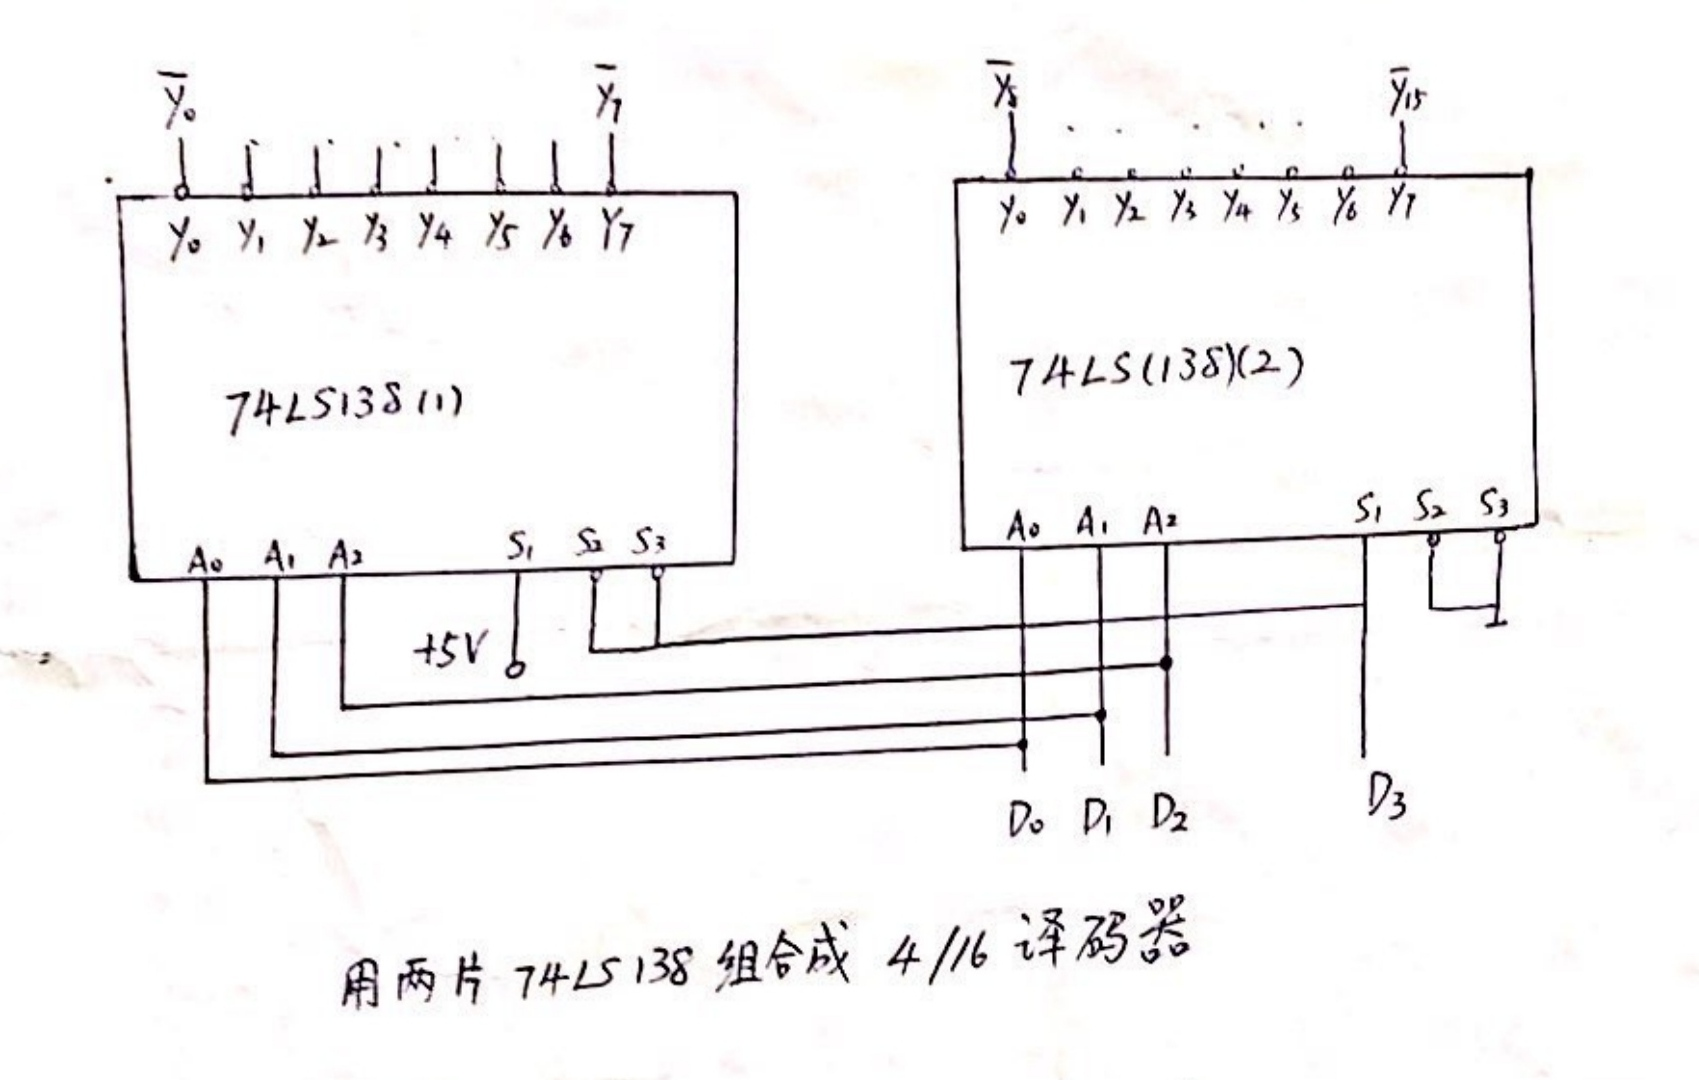
\includegraphics[scale=0.125]{1.jpg}
\caption{逻辑图}
\label{figure}
\end{figure}
\newpage

2.真值表

实验真值表如下:
\begin{table}[htbp]
	\centering
	\caption{True value table}
\resizebox{\textwidth}{!}{
\begin{tabular}{|c|c|c|c|c|c|c|c|c|c|c|c|c|c|c|c|c|c|c|c|}
	\hline
	$D_3$&$D_2$&$D_1$&$D_0$&$y_0$&$y_1$&$y_2$&$y_3$&$y_4$&$y_5$&$y_6$&$y_7$&$y_8$&$y_9$&$y_{10}$&$y_{11}$&$y_{12}$&$y_{13}$&$y_{14}$&$y_{15}$\\
	\hline
	0&0&0&0&0&1&1&1&1&1&1&1&1&1&1&1&1&1&1&1\\
\hline
	0&0&0&1&1&0&1&1&1&1&1&1&1&1&1&1&1&1&1&1\\
\hline
	0&0&1&0&1&1&0&1&1&1&1&1&1&1&1&1&1&1&1&1\\
\hline
	0&0&1&1&1&1&1&0&1&1&1&1&1&1&1&1&1&1&1&1\\
\hline
	0&1&0&0&1&1&1&1&0&1&1&1&1&1&1&1&1&1&1&1\\
\hline
	0&1&0&1&1&1&1&1&1&0&1&1&1&1&1&1&1&1&1&1\\
\hline
	0&1&1&0&1&1&1&1&1&1&0&1&1&1&1&1&1&1&1&1\\
\hline
	0&1&1&1&1&1&1&1&1&1&1&0&1&1&1&1&1&1&1&1\\
\hline
	1&0&0&0&1&1&1&1&1&1&1&1&0&1&1&1&1&1&1&1\\
\hline
	1&0&0&1&1&1&1&1&1&1&1&1&1&0&1&1&1&1&1&1\\
\hline
	1&0&1&0&1&1&1&1&1&1&1&1&1&1&0&1&1&1&1&1\\
\hline
	1&0&1&1&1&1&1&1&1&1&1&1&1&1&1&0&1&1&1&1\\
\hline
	1&1&0&0&1&1&1&1&1&1&1&1&1&1&1&1&0&1&1&1\\
\hline
	1&1&0&1&1&1&1&1&1&1&1&1&1&1&1&1&1&0&1&1\\
\hline
	1&1&1&0&1&1&1&1&1&1&1&1&1&1&1&1&1&1&0&1\\
\hline
	1&1&1&1&1&1&1&1&1&1&1&1&1&1&1&1&1&1&1&0\\
	\hline	
\end{tabular}
}
\end{table}
\newpage

\section{实验结果}
仅使用一片芯片控制$y_0$至$y_7$时,当$S_1$为高电平且$S_2,S_3$均为低电平时,译码器可以将二进制译为十进制,对应小灯为暗。其余情况下,小灯全为亮。

用两片74LS138组合成一个4线-16线译码器,可以将二进制码译为十进制码,使对应的小灯变暗。当$D_1$为低电平时控制$y_0$至$y_7$的输出,$D_1$为高电平时控制$y_8$至$y_{15}$的输出。输出结果与真值表情况相同。

\section{实验总结}

通过这次实验,我初步掌握了组合线路的设计方法,学会使用2片3线-8线译码器搭建4线-16线译码器,加深了对相关理论知识的理解。

但是,在使用两片3线-8线芯片设计4线-16线芯片时,会使一个使能端失去作用,可以优化。

\end{document}